\documentclass[12pt]{article}

\usepackage[letterpaper,margin=1in]{geometry}

\setlength{\parindent}{0pt}

\usepackage{amssymb}
\usepackage{amsmath}

\usepackage{multicol}

\usepackage{tikz}

\newcommand{\headerText}{
  MA 237 | Spring 2018 | Dr. Clontz
}

\usepackage{fancyhdr}
\pagestyle{fancy}
\renewcommand{\headrulewidth}{0pt}% Default \headrulewidth is 0.4pt
\renewcommand{\footrulewidth}{0pt}% Default \footrulewidth is 0pt
\chead{\footnotesize\bf\headerText}
\cfoot{}

\newcommand{\csch}{\operatorname{csch}}
\newcommand{\sech}{\operatorname{sech}}

\newcommand{\issuesMark}{{\fontencoding{U}\fontfamily{futs}\selectfont\char 66\relax}}




\begin{document}


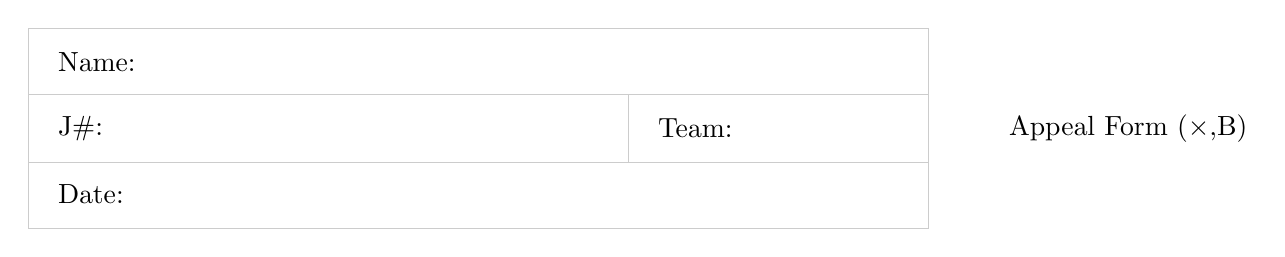
\begin{tikzpicture}[x=1in,y=1in]
  \draw[color=black!20] (0,0) rectangle (4.5,1);
  \draw[color=black!20] (0,0.67) -- (4.5,0.67);
  \draw[color=black!20] (3,0.33) -- (3,0.67);
  \draw[color=black!20] (0,0.33) -- (4.5,0.33);

  \node[anchor=west] at (0.1,0.83) {Name:};
  \node[anchor=west] at (0.1,0.5) {J\#:};
  \node[anchor=west] at (3.1,0.5) {Team:};
  \node[anchor=west] at (0.1,0.17) {Date:};

  \node at (5.5,0.5) {Appeal Form (\(\times\),\issuesMark{})};
\end{tikzpicture}

\vspace{1em}

\begin{tikzpicture}[x=1in,y=1in]
  \draw[color=black!50] (0,0) rectangle (6.4,1);
  \draw[color=black!50] (1,0) -- (1,1);
  \draw[color=black!50] (3.2,0) -- (3.2,1);
  \draw[color=black!50] (5.4,0) -- (5.4,1);

  \node[anchor=north west,color=black!70] at (0,0.95) {\footnotesize Standard:};
  \node[anchor=north west,color=black!70] at (1,0.95) {\footnotesize Mastery Quiz:};
  \node[anchor=north west,color=black!70] at (3.2,0.95) {\footnotesize Exercise Version:};
  \node[anchor=north west,color=black!70] at (5.4,0.95) {\footnotesize New mark:};
\end{tikzpicture}

This form should be submitted on the date
of the upcoming Mastery Quiz and counts as your submission for the
corresponding standard on that Quiz.

\vspace{1em}

Staple the originally marked Mastery Quiz exercise to this form.
Below, clearly explain why the error in your solution is unrelated to
your understanding of the relevant standard (e.g. explain your notation or
arithmetic error).
If your explanation is not satisfactory, this form will be marked with
\(\times\).

\vfill

Use the provided space to write a complete revised solution. You do not
need to rewrite the question.

\vfill


\vfill

\end{document}
